\documentclass[10pt]{article}  

%%%%%%%% PREÁMBULO %%%%%%%%%%%%
\title{Práctica 5 DSS}
\usepackage[spanish]{babel} %Indica que escribiermos en español
\usepackage[utf8]{inputenc} %Indica qué codificación se está usando ISO-8859-1(latin1)  o utf8  
\usepackage{amsmath} % Comandos extras para matemáticas (cajas para ecuaciones,
% etc)
\usepackage{amssymb} % Simbolos matematicos (por lo tanto)
\usepackage{graphicx} % Incluir imágenes en LaTeX
\usepackage{color} % Para colorear texto
\usepackage{subfigure} % subfiguras
\usepackage{float} %Podemos usar el especificador [H] en las figuras para que se
% queden donde queramos
\usepackage{capt-of} % Permite usar etiquetas fuera de elementos flotantes
% (etiquetas de figuras)
\usepackage{sidecap} % Para poner el texto de las imágenes al lado
	\sidecaptionvpos{figure}{c} % Para que el texto se alinie al centro vertical
\usepackage{caption} % Para poder quitar numeracion de figuras
\usepackage{commath} % funcionalidades extras para diferenciales, integrales,
% etc (\od, \dif, etc)
\usepackage{cancel} % para cancelar expresiones (\cancelto{0}{x})
 
\usepackage{anysize} 					% Para personalizar el ancho de  los márgenes
\marginsize{2cm}{2cm}{2cm}{2cm} % Izquierda, derecha, arriba, abajo

\usepackage{appendix}
\renewcommand{\appendixname}{Apéndices}
\renewcommand{\appendixtocname}{Apéndices}
\renewcommand{\appendixpagename}{Apéndices} 

% Para que las referencias sean hipervínculos a las figuras o ecuaciones y
% aparezcan en color
\usepackage[colorlinks=true,plainpages=true,citecolor=blue,linkcolor=blue]{hyperref}
%\usepackage{hyperref} 
% Para agregar encabezado y pie de página
\usepackage{fancyhdr} 
\pagestyle{fancy}
\fancyhf{}
\fancyhead[L]{\footnotesize UGR} %encabezado izquierda
\fancyhead[R]{\footnotesize LSI}   % dereecha
\fancyfoot[R]{\footnotesize Práctica 5}  % Pie derecha
\fancyfoot[C]{\thepage}  % centro
\fancyfoot[L]{\footnotesize Master en Ingeniería Informática}  %izquierda
\renewcommand{\footrulewidth}{0.4pt}


\usepackage{listings} % Para usar código fuente
\definecolor{dkgreen}{rgb}{0,0.6,0} % Definimos colores para usar en el código
\definecolor{gray}{rgb}{0.5,0.5,0.5} 
% configuración para el lenguaje que queramos utilizar
\lstset{language=Matlab,
   keywords={break,case,catch,continue,else,elseif,end,for,function,
      global,if,otherwise,persistent,return,switch,try,while},
   basicstyle=\ttfamily,
   keywordstyle=\color{blue},
   commentstyle=\color{red},
   stringstyle=\color{dkgreen},
   numbers=left,
   numberstyle=\tiny\color{gray},
   stepnumber=1,
   numbersep=10pt,
   backgroundcolor=\color{white},
   tabsize=4,
   showspaces=false,
   showstringspaces=false}

\newcommand{\sen}{\operatorname{\sen}}	% Definimos el comando \sen para el seno
%en español

\title{Desarrollo completo de una aplicación interactiva para dispositivos móviles}

%%%%%%%% TERMINA PREÁMBULO %%%%%%%%%%%%

\begin{document}

%%%%%%%%%%%%%%%%%%%%%%%%%%%%%%%%%% PORTADA %%%%%%%%%%%%%%%%%%%%%%%%%%%%%%%%%%%%%%%%%%%%
																					%%%
\begin{center}																		%%%
\newcommand{\HRule}{\rule{\linewidth}{0.5mm}}									%%%\left
 																					%%%
\begin{minipage}{0.48\textwidth} \begin{flushleft}
%
\includegraphics[scale = 0.63]{Imagenes/logo_upiita}
\end{flushleft}\end{minipage}
\begin{minipage}{0.48\textwidth} \begin{flushright}
%
\includegraphics[scale = 0.35]{Imagenes/IPN}
\end{flushright}\end{minipage}

													 								%%%
\vspace*{-1.5cm}								%%%
																					%%%	
\textsc{\huge Universidad de\\ \vspace{5px} Granada}\\[1.5cm]	

\textsc{\LARGE Desarrollo de Sistemas Software\\ \vspace{5px}  Basados en Componentes}\\[1.5cm]													%%%

\begin{minipage}{0.9\textwidth} 
\begin{center}																					%%%
\textsc{\LARGE Práctica 5}
\end{center}
\end{minipage}\\[0.5cm]
%%%
    																				%%%
 			\vspace*{1cm}																		%%%
																					%%%
\HRule \\[0.4cm]																	%%%
{ \huge \bfseries Desarrollo completo de una aplicación interactiva para dispositivos móviles}\\[0.4cm]	%%%
 																					%%%
\HRule \\[1.5cm]																	%%%
 																				%%%
																					%%%
\begin{minipage}{0.46\textwidth}													%%%
\begin{flushleft} \large															%%%
\emph{Autor:}\\	
Manuel Jesús García Manday\\

%%%
			%\vspace*{2cm}	
            													%%%
										 						%%%
\end{flushleft}																		%%%
\end{minipage}		
																%%%
\begin{minipage}{0.52\textwidth}		
\vspace{-0.6cm}											%%%
\begin{flushright} \large															%%%
													%%%
\end{flushright}																	%%%
\end{minipage}	
\vspace*{1cm}
%\begin{flushleft}
 	
%\end{flushleft}
%%%
 		\flushleft{\textbf{\Large Master en Ingeniería Informática}	}\\																		%%%
\vspace{2cm} 																				
\begin{center}																					
%{\large \today}																	%%%
 			\end{center}												  						
\end{center}							 											
																					
\newpage																		
%%%%%%%%%%%%%%%%%%%% TERMINA PORTADA %%%%%%%%%%%%%%%%%%%%%%%%%%%%%%%%

\tableofcontents 

\newpage

\section{Objetivo.}



El objetivo de esta quinta práctica de la asignatura es desarrollar una aplicación interactiva para dispositivos móviles que cumpla con una serie de requisitos funcionales y no funcionales, de acorde al contenido de la asignatura y al temario relacionado con esta practica.



\section{Objetivos de la aplicación.} 

El juego que se tiene que desarrollar ha de poder ejecutarse en un dispositivo Android (versión >= 4.4) o IOS (elegir sólo uno) y se trata de presentar una serie de preguntas al usuario, que tendrá que responder para alcanzar una puntuación global, así como el número de respuestas acertadas y falladas. \\

Se tendrá una primera pantalla de presentación con un botón para iniciar el juego, otro para obtener los resultados y estadísticas obtenidos después de jugar y un tercer botón para enlazar con juegos similares libres que existan en Internet y que se puedan utilizar desde un tipo de aplicación como la que se pretende desarrollar.\\

Cada pantalla del juego ha de consistir en 1 pregunta con 4 posibles respuestas alternativas; la pregunta podría ser un texto plano, o una pregunta que contenga imágenes y sonidos.\\

Se ha de construir una base de datos de preguntas de texto planas a la que acceda directamente la app, de tal forma que en el futuro se puedan cambiar las preguntas de texto sin tener que modificar el código de la citada aplicación, aunque haya que volver a generar el archivo apk desplegable.\\

Al seleccionar una de las respuestas en cada pregunta ha de aparecer un mensaje de felicitación en el pie de la pantalla junto con un sonido de acierto o fallo; después de unos segundos se pasará a la siguiente pantalla con otra pregunta.\\

En caso de no acertar, se ha de poder elegir entre volver a la pantalla inicial para comenzar de nuevo el juego y se obtendrá un mensaje con la respuesta correcta o bien continuar el juego (no se obtendría las soluciones hasta el final); en ambos casos, se pueden obtener los resultados acumulados durante el desarrollo de un juego volviendo a la pantalla de inicio y pulsando e el botón "Resultados".\\

Tras la última pregunta, el mensaje que se mostrará será de felicitación por haber realizado el juego y mensaje de despedida antes de volver a iniciar el juego.\\


\section{Requisitos funcionales.}

Para que la aplicación desarrollada sea evaluada favorablemente ha de satisfacer los siguientes requisitos funcionales:\\

\begin{itemize}
	\item El juego deberá mostrar una batería de preguntas.
	\item El usuario ha de poder responder a las preguntas de una en una.
	\item Si el usuario falla la pregunta, se le mostrará un mensaje indicándole que ha fallado junto con un sonido.
	\item Si el usuario acierta,se le muestra un mensaje indicándole que ha acertado.
	\item Ha de haber pantallas de pregunta que incluyan 1 imagen
	\item Si el usuario falla, entonces deberá aparecer la opción de continuar la partida o de volver a iniciar el juego.
	\item Si el usuario acierta, continuará con la siguiente pregunta.
	\item Cuando el usuario finaliza la partida, se le muestran los resultados que ha obtenido. 
	\item El menú deberá poder dirigirnos, al inicio de una nueva partida, a una opción que nos permita ver los resultados obtenidos en las partidas realizadas anteriormente, o a otros juegos en la Red mediante un webView.

\end{itemize}


\section{Requisitos no funcionales.}

Para que la aplicación desarrollada sea evaluada favorablemente ha de satisfacer los siguientes requisitos no funcionales:\\

\begin{itemize}
	\item Solamente puede hacerse un único acceso a la base de datos.
	\item La aplicación deberá funcionar como mínimo en dispositivos con versiones de sistemas
operativos actuales, en nuestro caso para dispositivos con veriones  de Android >=4.2.
	\item La aplicación debe funcionar tanto en dispositivos móviles (teléfonos) como en tablets.
	\item Se debe desarrollar la aplicación pedida aplicando Patrones de Diseño Software (por ejemplo: Singleton, Inmutable, Proxy, Escuchador de Eventos ) y Patrones Arquitectónicos (por ejemplo: MVC, DataBaseManagement System).

\end{itemize}


\section{Desarrollo del sistema.}

El desarrollo de la aplicación interactiva se ha realizado para dispositivos con Android debido a la mayor cuota de mercado que esta plataforma regenta. Como herramienta de desarrollo se ha utilizado el IDE Visual Studio junto con la versión 24 del SDK, aunque la aplicación es retrocompatible con versiones anteriores (hasta la SDK 16 en este caso).

El esquema de la aplicación es el que se muestra a continuación:



\begin{figure}[H]
	\begin{center}
 		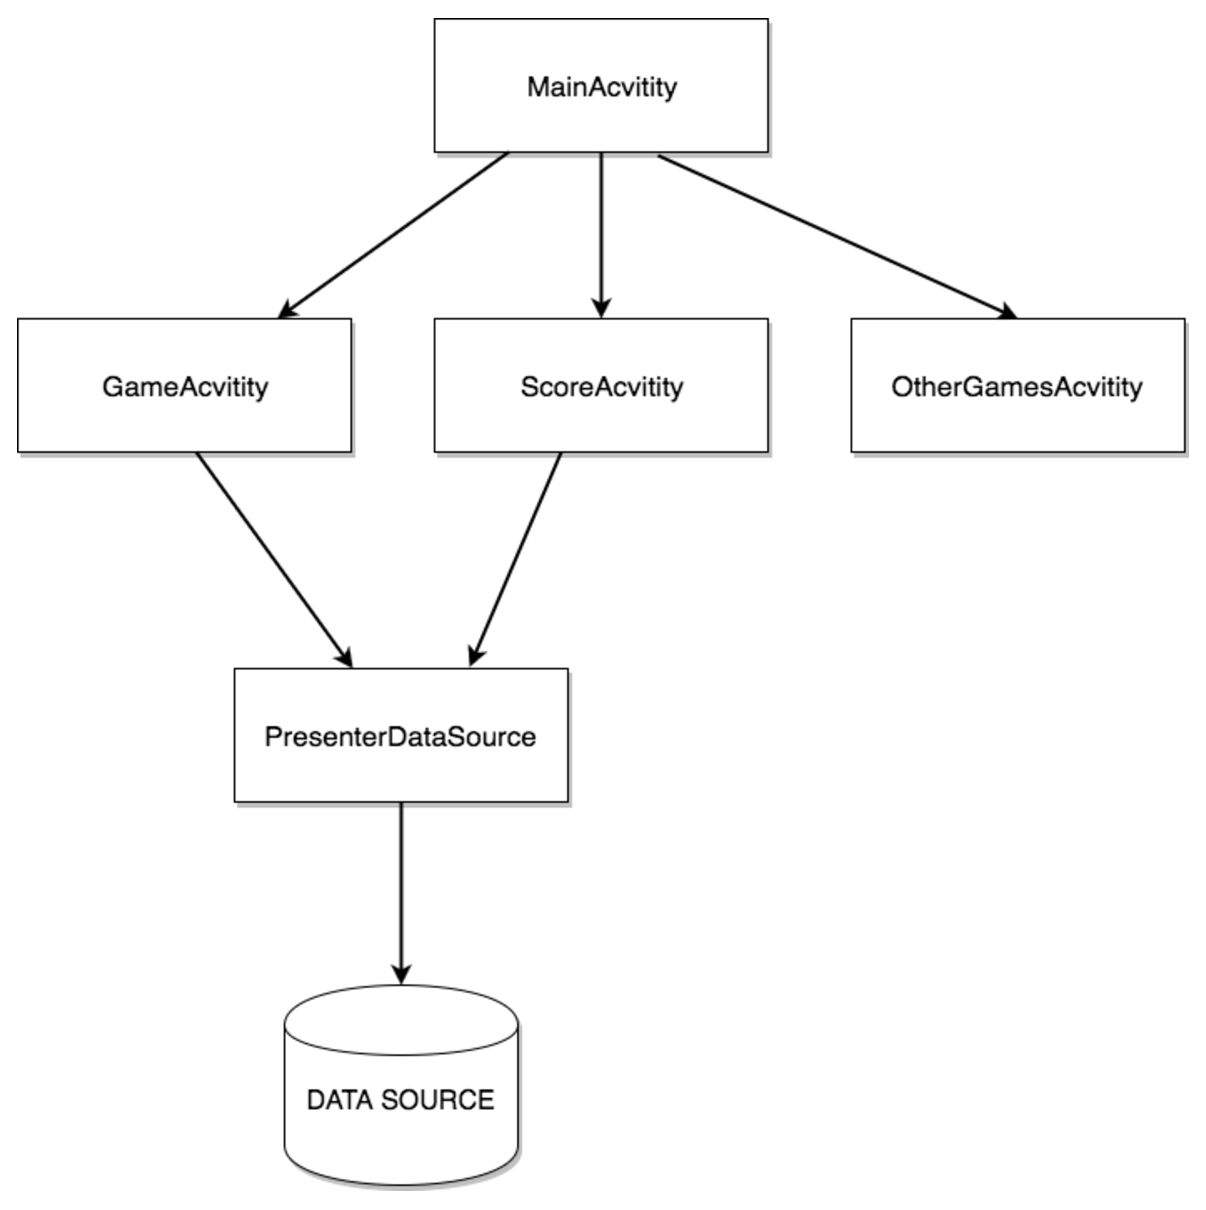
\includegraphics[width = 0.5\textwidth]{Imagenes/arquitectura.eps}
 		\captionof{figure}{\label{fig:IPN}Patrón arquitectónico} 
	\end{center} 
\end{figure}

Como se puede ver a través de la imagen, la fuente de datos (data source) es totalmente independiente de las actividades que la necesitan, consiguiendo de esta forma un alto grado de desacoplamiento que permite cualquier tipo de cambio, como por ejemplo que la base de datos se encuentre en un servidor en la nube y no en local como es nuestro caso, o que se utilice otro motor de base de datos que no sea SQLite como el que usamos. Implementado este patrón de diseño, la vista y la lógica de la misma quedan desligadas de los datos, teniendo sólo que modificar la lógica que implemente al Presenter. 

Este tipo de patrón de diseño permite abstraer la vista y el controlador del módelo, consiguiendo con ello que la aplicación sea escalable además de reutilizable.

Para cumplir con todos los objetivos propuestos, se ha implementado varios de los patrones de diseño y arquitectónicos como se puede también comprobar en el diagrama de clases de la aplicación.

\begin{figure}[H]
	\begin{center}
 		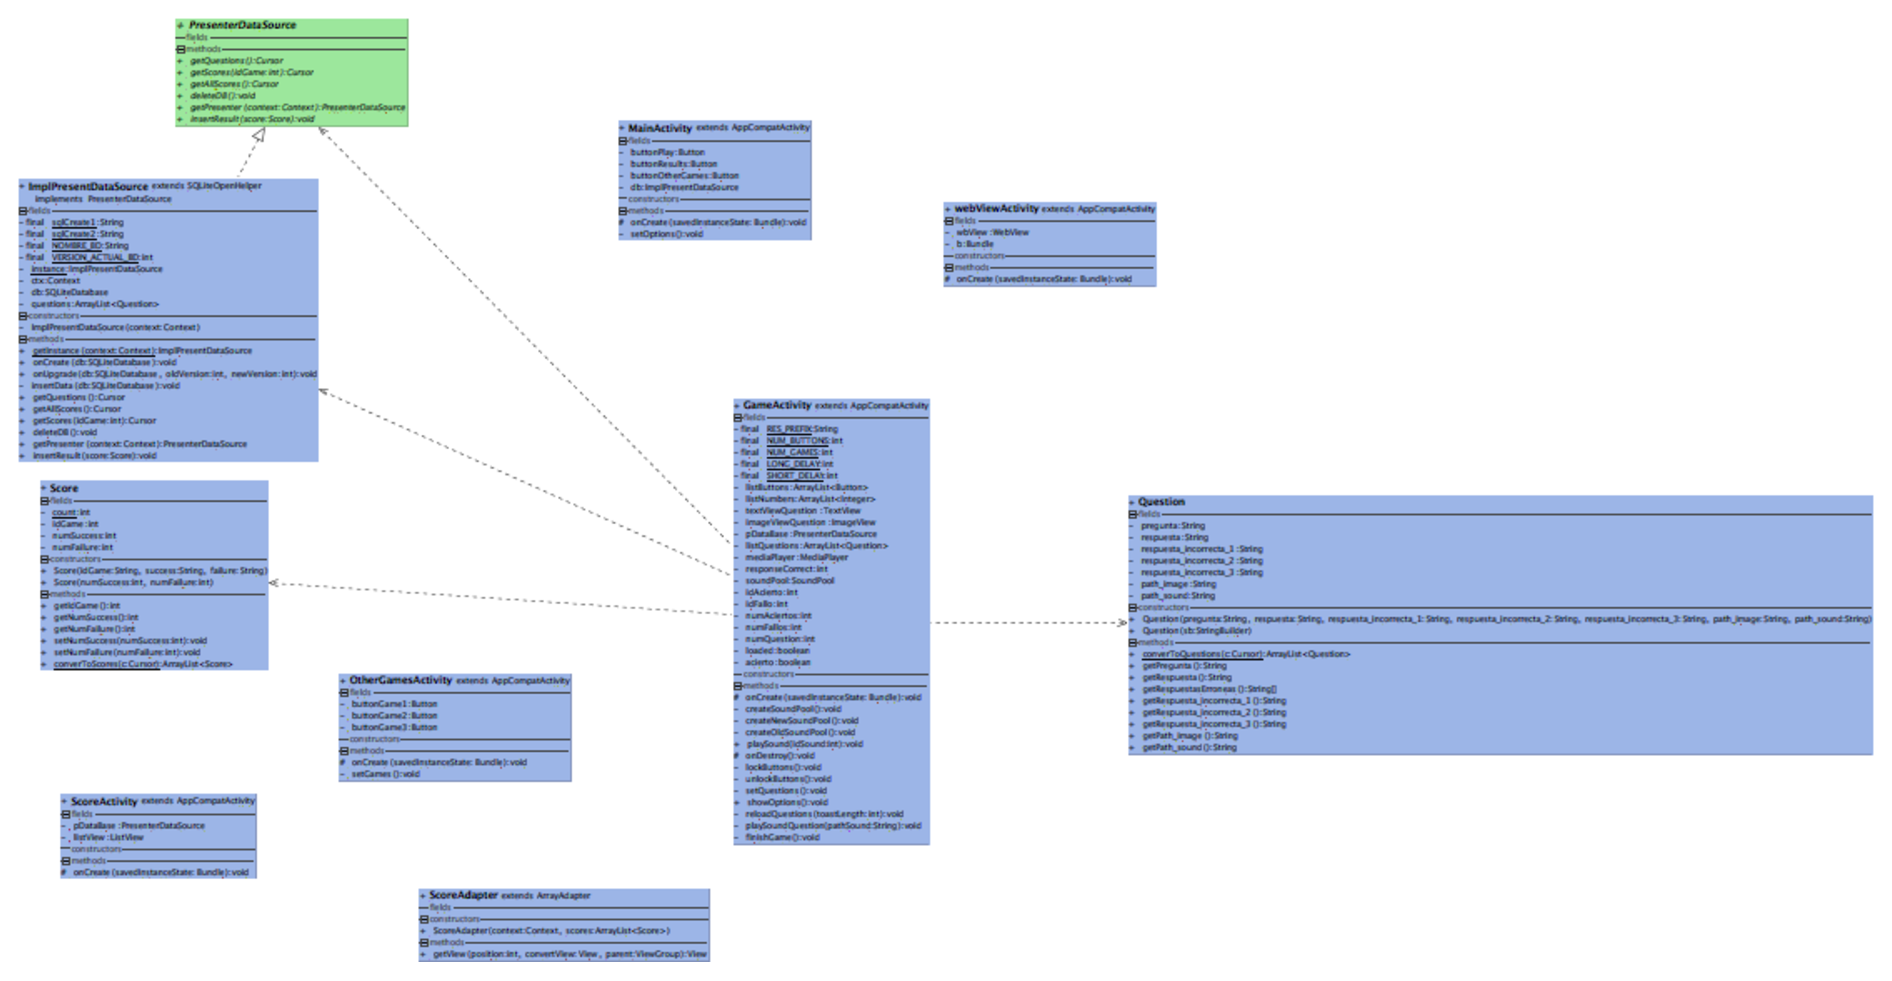
\includegraphics[width = 1.05\textwidth]{Imagenes/diagramaClases.eps}
 		\captionof{figure}{\label{fig:IPN}Diagrama de clases} 
	\end{center} 
\end{figure}


\subsection{El juego.}

Como se muestra en las indicaciones, el juego consta de una batería de preguntas con texto, imágenes y sonido, las cuales tienen cuatro posibles respuestas siendo sólo una la verdadera. Por defecto, el juego está configurado para que el ciclo de preguntas a contestar en una partida es de siete, aunque este parámetro es modificable.

Si la respuesta es la correcta se reproduce el sonido de acierto y se pasa a la siguiente pregunta después de unos segundos, y si por el contrario la respuesta es errónea el juego te da la opción de continuar o volver al inicio, al continuar pasará a la siguiente pregunta tras unos segundos mientras muestra un mensaje con la respuesta correcta.

En cualquier momento del juego se puede consultar la puntuación volviendo a la pantalla de inicio, una vez que se vuelve a esa pantalla el juego se da por terminado y la puntuación para esa partida será grabada en la base de datos.

La tercera opción de la pantalla principal permite ejecutar tres juegos diferentes de una plataforma online, los cuales son posibles jugar desde el dispositivo sin necesidad de configurar ni actualizar nada.

\begin{figure}[H]
	\begin{center}
 		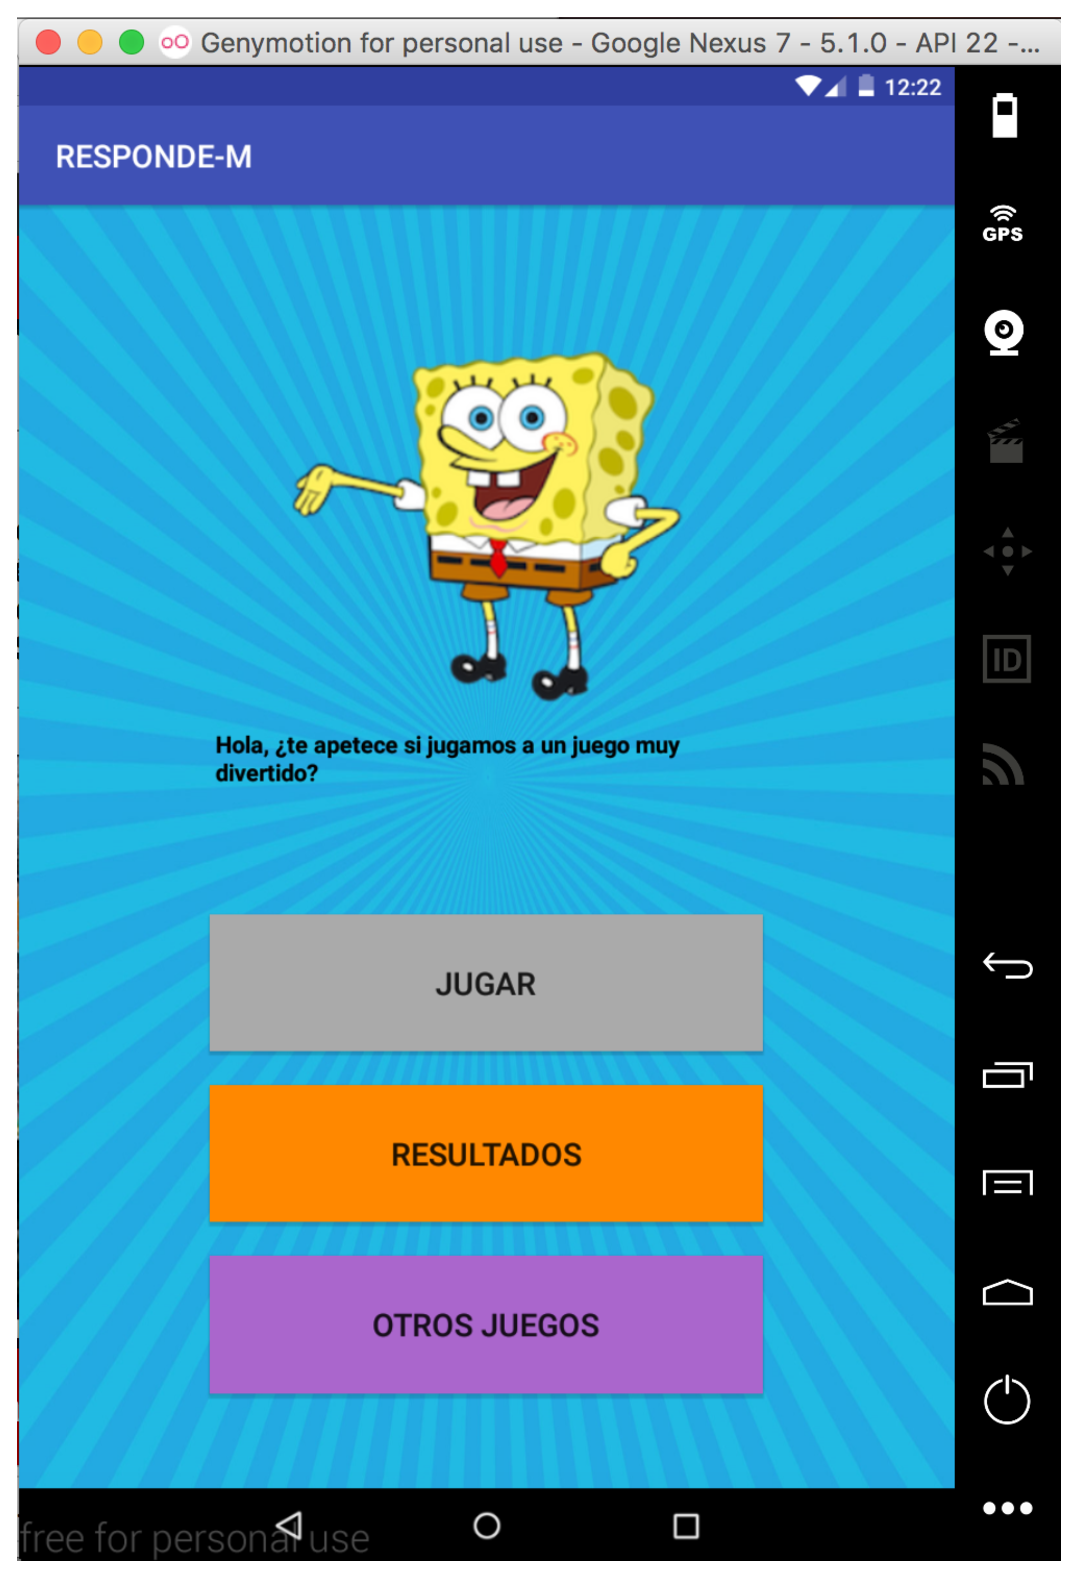
\includegraphics[width = 0.8\textwidth]{Imagenes/captura1.eps}
 		\captionof{figure}{\label{fig:IPN}Pantalla principal del juego.} 
	\end{center} 
\end{figure}

\begin{figure}[H]
	\begin{center}
 		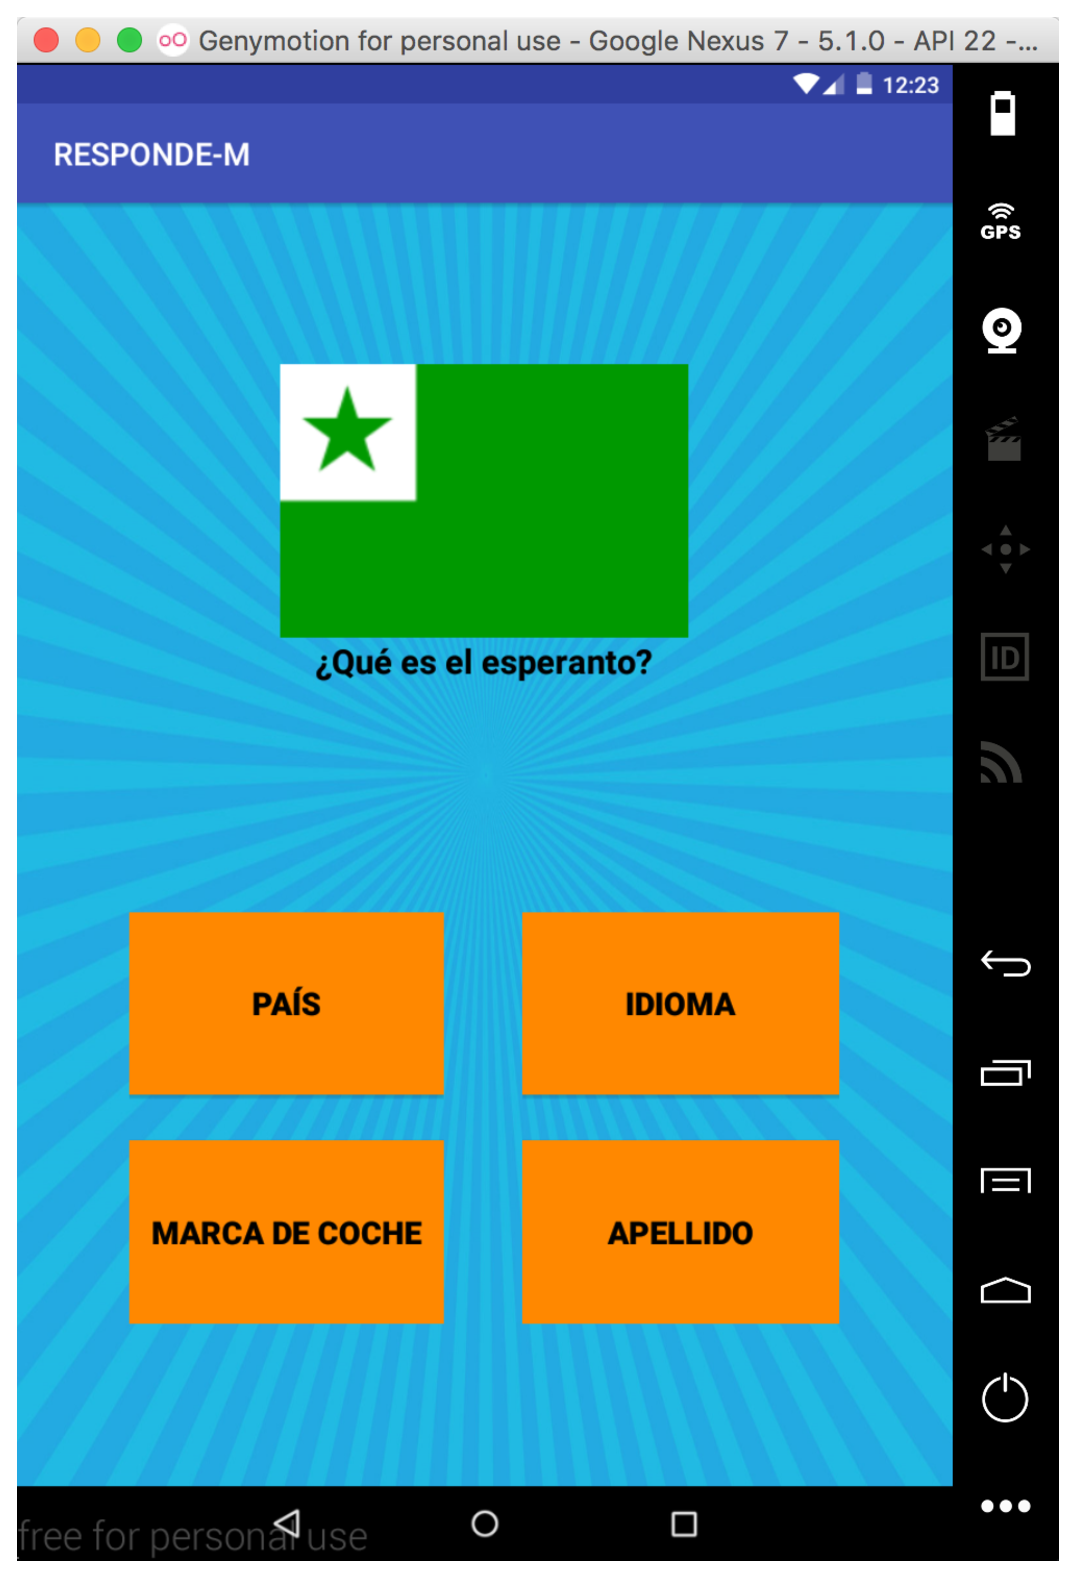
\includegraphics[width = 0.8\textwidth]{Imagenes/captura2.eps}
 		\captionof{figure}{\label{fig:IPN}Pantalla del juego de preguntas.} 
	\end{center} 
\end{figure}

\begin{figure}[H]
	\begin{center}
 		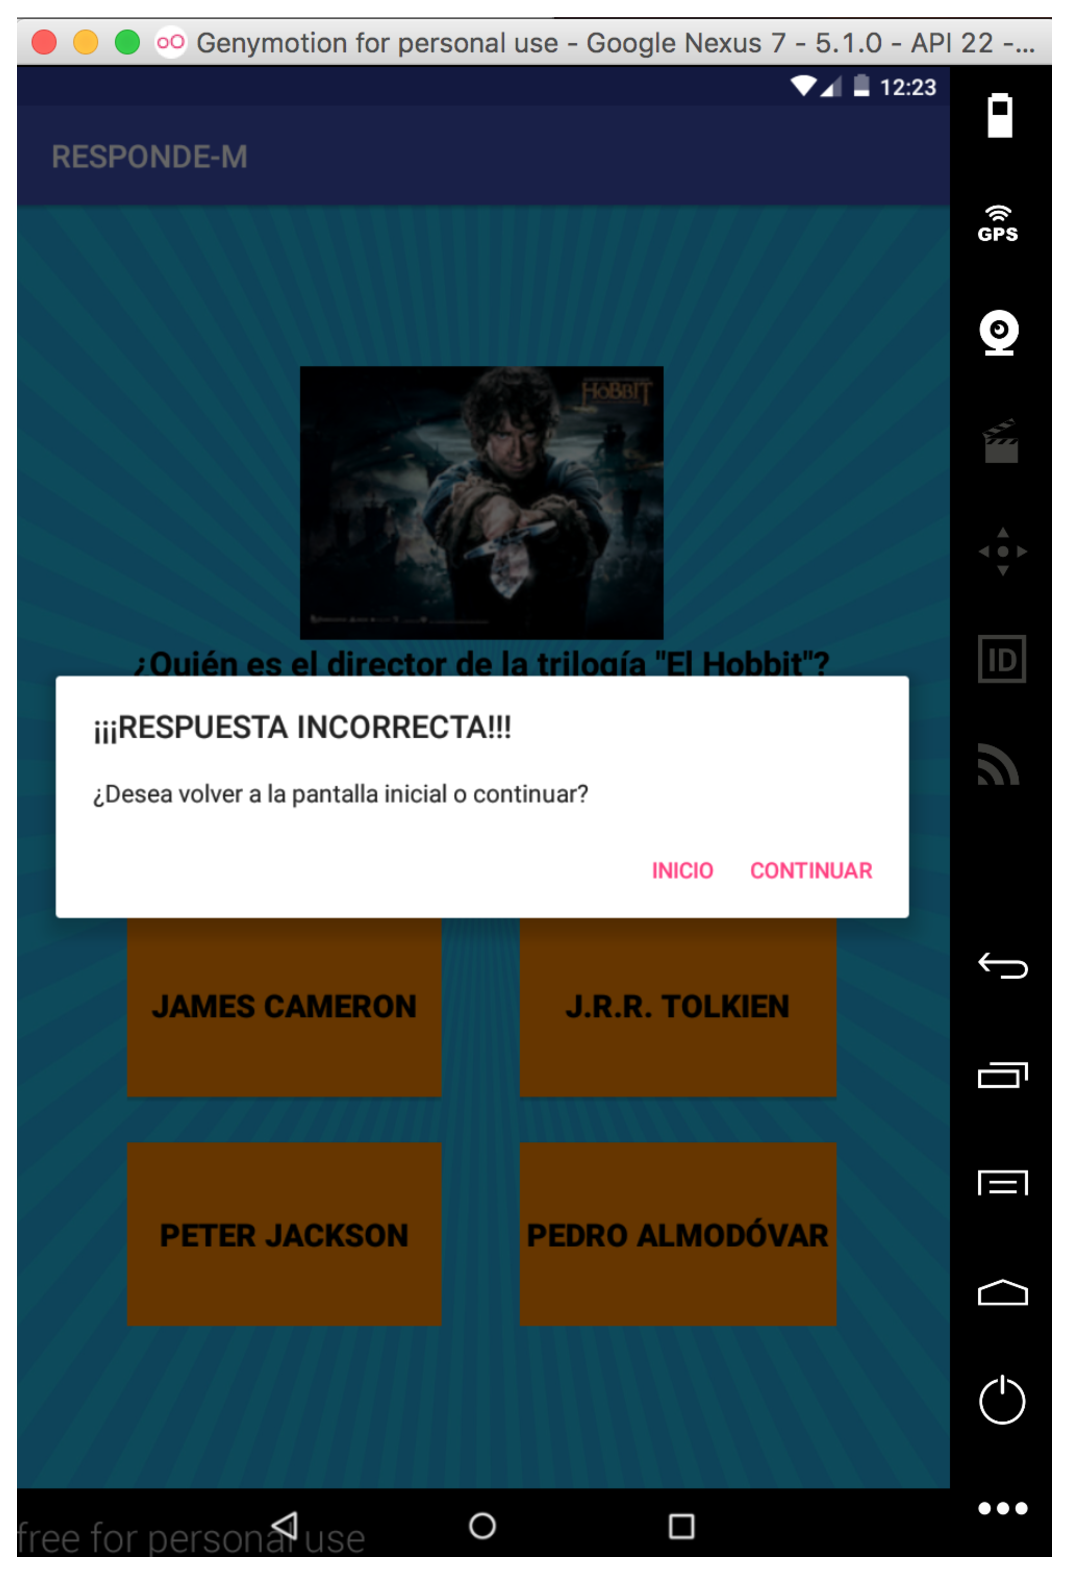
\includegraphics[width = 0.8\textwidth]{Imagenes/captura3.eps}
 		\captionof{figure}{\label{fig:IPN}Pantalla de opciones tras errar una respuesta.} 
	\end{center} 
\end{figure}

\begin{figure}[H]
	\begin{center}
 		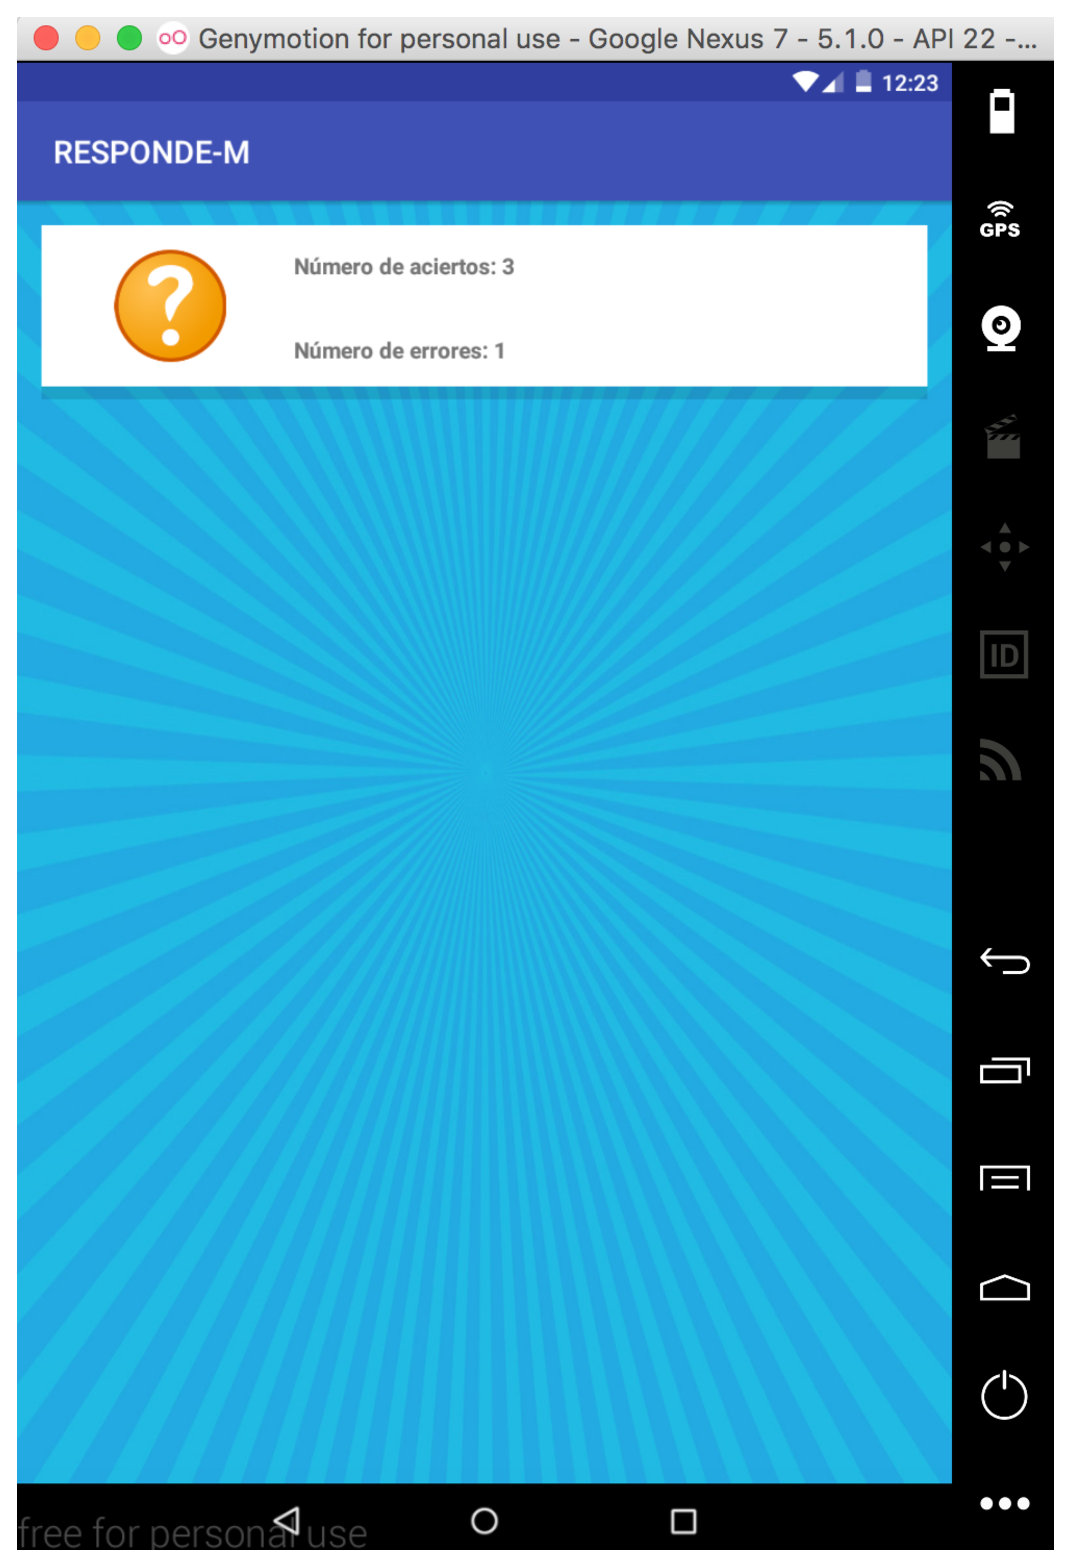
\includegraphics[width = 0.8\textwidth]{Imagenes/captura4.eps}
 		\captionof{figure}{\label{fig:IPN}Patanlla de las puntuaciones.} 
	\end{center} 
\end{figure}

\begin{figure}[H]
	\begin{center}
 		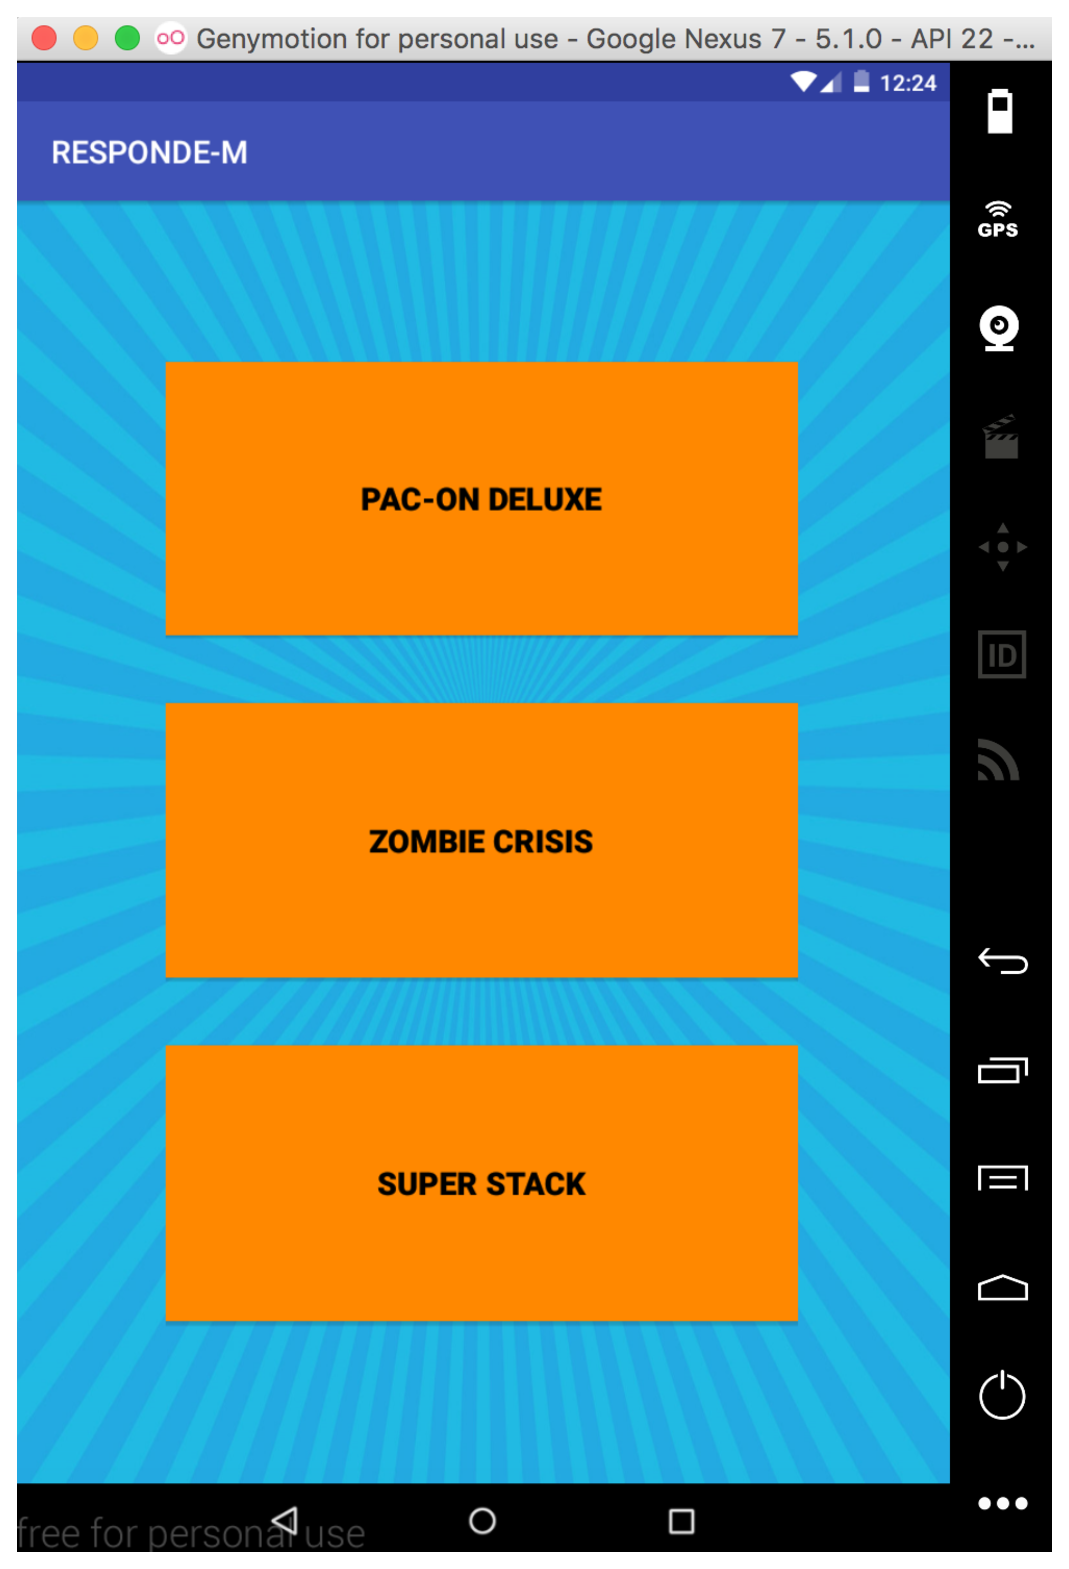
\includegraphics[width = 0.8\textwidth]{Imagenes/captura5.eps}
 		\captionof{figure}{\label{fig:IPN}Pantalla de los juegos on-line.} 
	\end{center} 
\end{figure}

\begin{figure}[H]
	\begin{center}
 		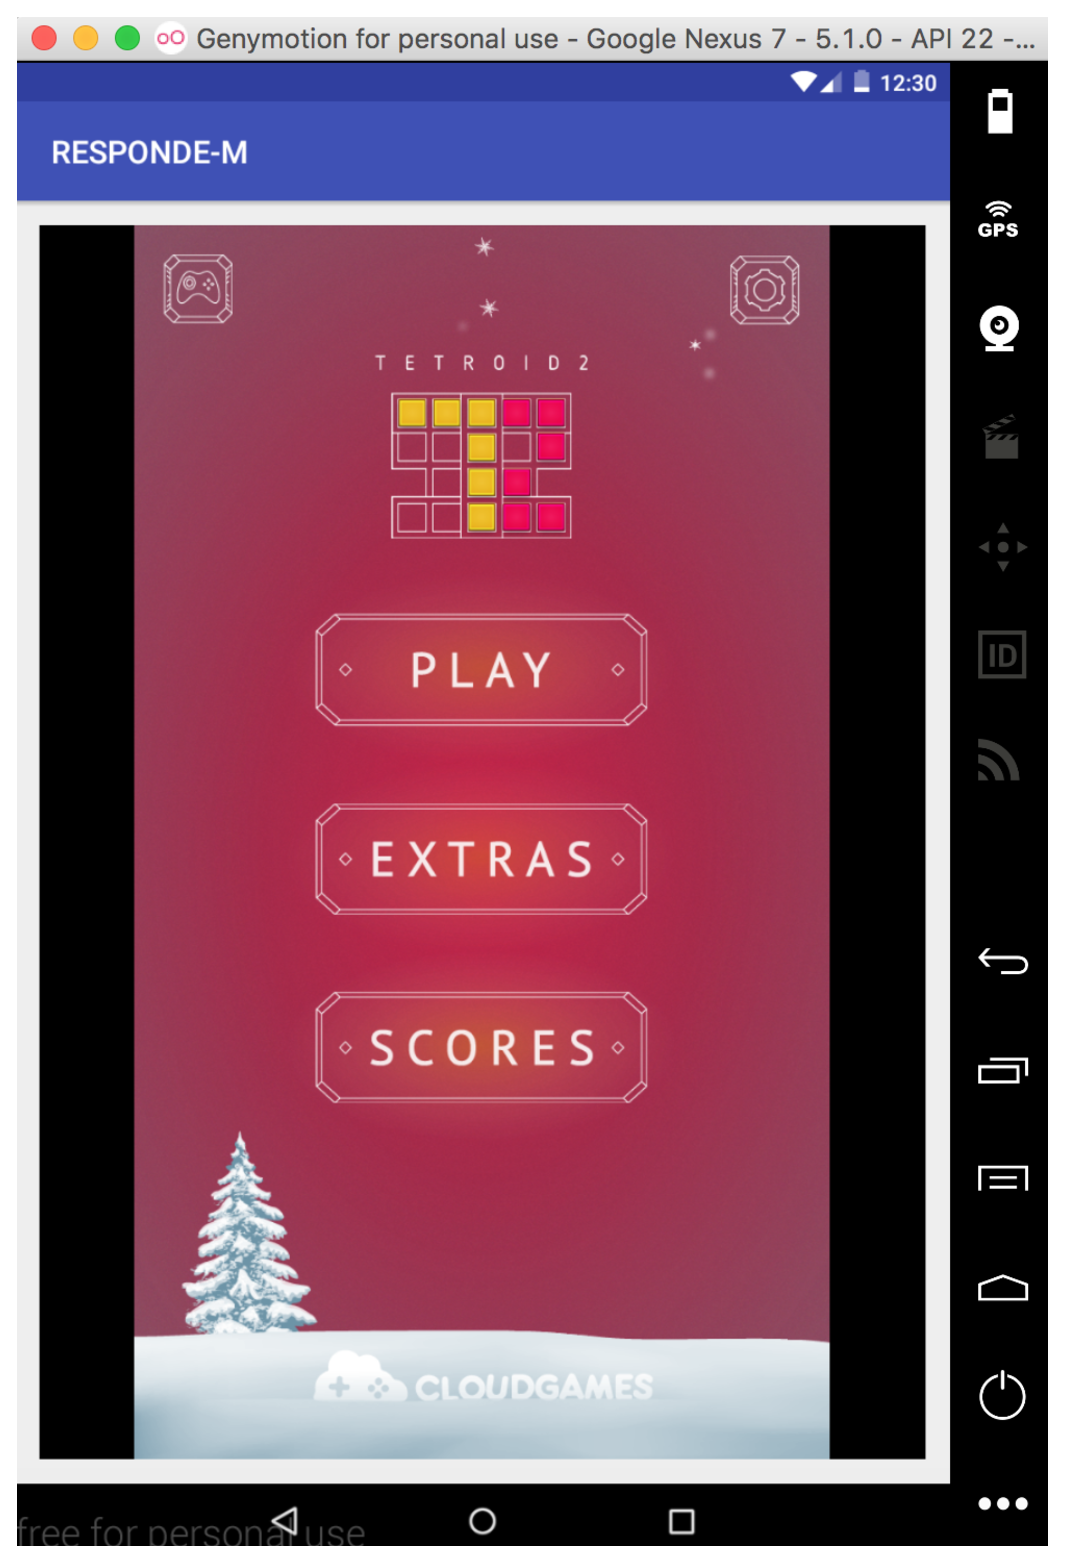
\includegraphics[width = 0.8\textwidth]{Imagenes/captura6.eps}
 		\captionof{figure}{\label{fig:IPN}Pantalla de un juego on-line.} 
	\end{center} 
\end{figure}

La aplicación cumple con todos los requisitos funcionales y no funcionales requeridos al inicio del desarrollo de la práctica como se ha podido ver en este documento y como se puede comprobar ejecutando el juego. 

En el siguiente \href{https://consigna.ugr.es/g/LyX7JFBZBCqNw4WG/GarciaMandayJesus-p5.zip}{enlace} se encuentra el código de la aplicación. 


\end{document}